Offline replay cannot show what \emph{adjust LR} does, so we ran the full system, agents and executor included, on the 12 configurations of seed 2 with the gate trained only on seeds 0 and 1, and compared each controlled run with its uncontrolled counterpart (same seed and settings). Fig.~\ref{fig:closed} shows the result.

\begin{figure*}[t]
\centering
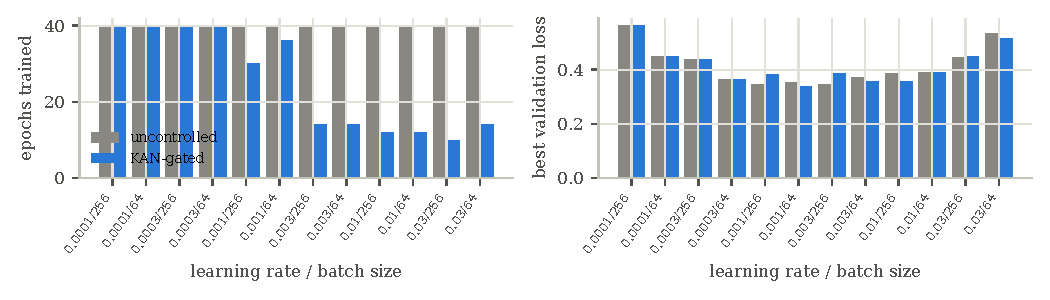
\includegraphics[width=0.85\textwidth]{figures/closed_loop.pdf}
\caption{Closed-loop control on 12 held-out configurations: epochs trained (left) and best validation loss (right), uncontrolled versus KAN-gated.}
\label{fig:closed}
\end{figure*}

The controlled runs used 302 of 480 epochs (37.1\% saved). Best validation loss was unchanged in aggregate: the median relative change was 0.0\% and the mean $+0.30\%$ (Wilcoxon $p=0.95$), with mean validation accuracy $+0.10$ points. Four runs improved by more than 0.5\%, all of them runs whose learning rate the gate had reduced (up to $-7.2\%$ at learning rate $10^{-2}$, batch 256); three got worse, two by $+10.6\%$ and $+11.1\%$ when a run that would still have improved was stopped after repeated reductions; five changed by less than 0.5\%. Low-learning-rate runs were left to finish.

Two behaviours are worth reporting. First, actuation latency: each controlled trajectory matched its uncontrolled twin exactly until one epoch after the first intervention, confirming that asynchronous control acts at the next epoch boundary. Second, the gate re-issues \emph{adjust LR} at consecutive checks while its score stays in the middle band, so the executor halved the learning rate up to ten times in one run. A cooldown between adjustments, or a gate input for recent interventions, is a straightforward fix that we leave to future work.
